% beautiful title slides in Beamer
% Model 6
% latex-beamer.com

\documentclass[aspectratio=169]{beamer}

\usepackage{media9}
\usepackage[backend=bibtex, style=authoryear, doi=false,isbn=false,url=false]{biblatex}
\usepackage[most]{tcolorbox}
\usepackage{subcaption}
\usepackage{bm}
\usepackage{diffcoeff}

% Math macros
\DeclareMathOperator*{\grad}{grad}
\DeclareMathOperator*{\Grad}{Grad}
\DeclareMathOperator*{\Div}{Div}
\renewcommand{\div}{\operatorname{div}}
\DeclareMathOperator*{\Hess}{Hess}
\DeclareMathOperator*{\curl}{curl}
\DeclareMathOperator{\Tr}{Tr}
\DeclareMathOperator{\Dom}{Dom}
\DeclareMathOperator*{\esssup}{ess\,sup}

\newcommand{\bbR}{\mathbb{R}}
\newcommand{\bbF}{\mathbb{F}}
\newcommand{\bbA}{\mathbb{A}}
\newcommand{\bbB}{\mathbb{B}}
\newcommand{\bbS}{\mathbb{S}}

\newcommand*{\norm}[1]{\ensuremath{\left\|#1\right\|}}
\newcommand{\where}{\qquad \text{where} \qquad}
\newcommand{\inner}[3][]{\ensuremath{\left\langle #2, \, #3 \right\rangle_{#1}}}
\newcommand{\bilprod}[2]{\left\langle \left\langle \, #1, #2 \, \right\rangle \right\rangle}
\newcommand{\pder}[2]{\ensuremath{\partial_{#2} #1}}
\newcommand{\dder}[2]{\ensuremath{\delta_{#2} #1}}
\newcommand{\secref}[1]{\S\ref{#1}}
\newcommand{\energy}[1]{\frac{1}{2} \int_{\Omega} \left\{ #1 \right\} \d\Omega}
\newcommand{\crmat}[1]{\ensuremath{\left[#1\right]_\times}}
\newcommand{\fenics}{\textsc{FEniCS}\xspace}
\newcommand{\firedrake}{\textsc{Firedrake}\xspace}


% Remove navigation bar
%\setbeamertemplate{navigation symbols}{}
\addtobeamertemplate{navigation symbols}{}{%
	\usebeamerfont{footline}%
	\usebeamercolor[fg]{footline}%
	\hspace{1em}%
	\insertframenumber/\inserttotalframenumber
}

\usepackage{color}
\definecolor{theme}{RGB}{0,73,114}

\setbeamertemplate{blocks}[rounded][shadow]

\setbeamercolor{block body alerted}{bg=alerted text.fg!10}
\setbeamercolor{block title alerted}{bg=alerted text.fg!20}
\setbeamercolor{block body}{bg=structure!10}
\setbeamercolor{block title}{bg=structure!20}
\setbeamercolor{block body example}{bg=green!10}
\setbeamercolor{block title example}{bg=green!20}
% Tikz package
\usepackage{tikz}
\usetikzlibrary{positioning}


\graphicspath{{./images/}}

\bibliography{biblio}


%% At begin of each section: show current section and all subsections in the section if any
%% At begin of each subsection except first: show only the current section/subsection
\newif\iftocsub
\tocsubtrue
\AtBeginSection[] {
	\begin{frame}[noframenumbering]{Outline}
		\tableofcontents[sectionstyle=show/shaded, subsectionstyle=show/show/hide]
	\end{frame}
	\tocsubfalse
}
\AtBeginSubsection[] {
	\iftocsub
	\begin{frame}[noframenumbering]{Outline}
		\tableofcontents[currentsubsection, sectionstyle=show/shaded, subsectionstyle=show/shaded/hide]
	\end{frame}
	\fi
	\tocsubtrue
}


\begin{document}

% Title slide frame
\begin{frame}[plain]

%%%%%%%% Title slide details %%%%%%%%%%%%%%


% Background Image
\newcommand{\myBackground}
{
    
\includegraphics[height=1.02\paperheight,page=9]{beamerthemeutresources}
}

% Title
\newcommand{\myTitle}
{
    Numerics for the Portwings project
}

% Subtitle
\newcommand{\mySubTitle}
{
    Current develpments and outlook
}

% Author
\newcommand{\myAuthor}   
{
    Andrea Brugnoli
}

% Affiliation
\newcommand{\myAffiliate}
{
  
}

% Presentation Date
\newcommand{\myDate}   
{
    \today
}

% Logo
\newcommand{\myLogo}   
{
    
\includegraphics[width=3cm]{Logo.png}
}
%%%%%%%%%%%%%%%%%%%%%%%%%%%%%%%%%%%%


%%%%%%%%%% Title slide code %%%%%%%%%%%
\begin{tikzpicture}[remember picture,overlay]

% Background color

\fill[white] (current page.south west) rectangle (current page.north east);
% Background image
\node[above right,inner sep=0pt] at (current page.south west)
    {
        \myBackground
    };
    
% Title & Subtitle
\node
[
    above=0.5cm,
    align=center,
    draw=black!50,
    % rounded corners,
    double,
    double distance=0.1cm,
    double=blue!10,
    fill=yellow!10,
    inner xsep=15pt,
    inner ysep=10pt, 
    minimum width=0.7\textwidth,
    text width=0.6\textwidth
] (title) at (current page.center)
{
    \LARGE \myTitle  \\[5pt]
    \small \mySubTitle
};

% Author 
\node[ below=0.5cm] (author) at (title.south){\myAuthor};

% Author 
\node[ below=0.25cm ](affiliate) at (author.south){\small \myAffiliate};

% Date
\node[below=0.25] (date) at (affiliate.south){\large \myDate};

% Logo
\node
[
    below =0.25cm
] at (date.south)
{
    \myLogo
};

\end{tikzpicture}
    
\end{frame}

\begin{frame}{Overview}
	\tableofcontents
\end{frame}

\section{Introduction}

\begin{frame}{Vision for the portwings project}

\begin{block}{Main objective}
Use a unified port-Hamiltonian (pH) framework to model fluid-structure interactions.
\end{block}

If successful, the approach will: 
\begin{itemize}
	\item be competitive w.r.t. state of the art methods;
	\item pave the way to other multiphysical problems;
	\item serve for model reduction and control of complex systems.
\end{itemize}

\begin{figure}[t]
	\begin{subfigure}[t]{0.3\textwidth}
		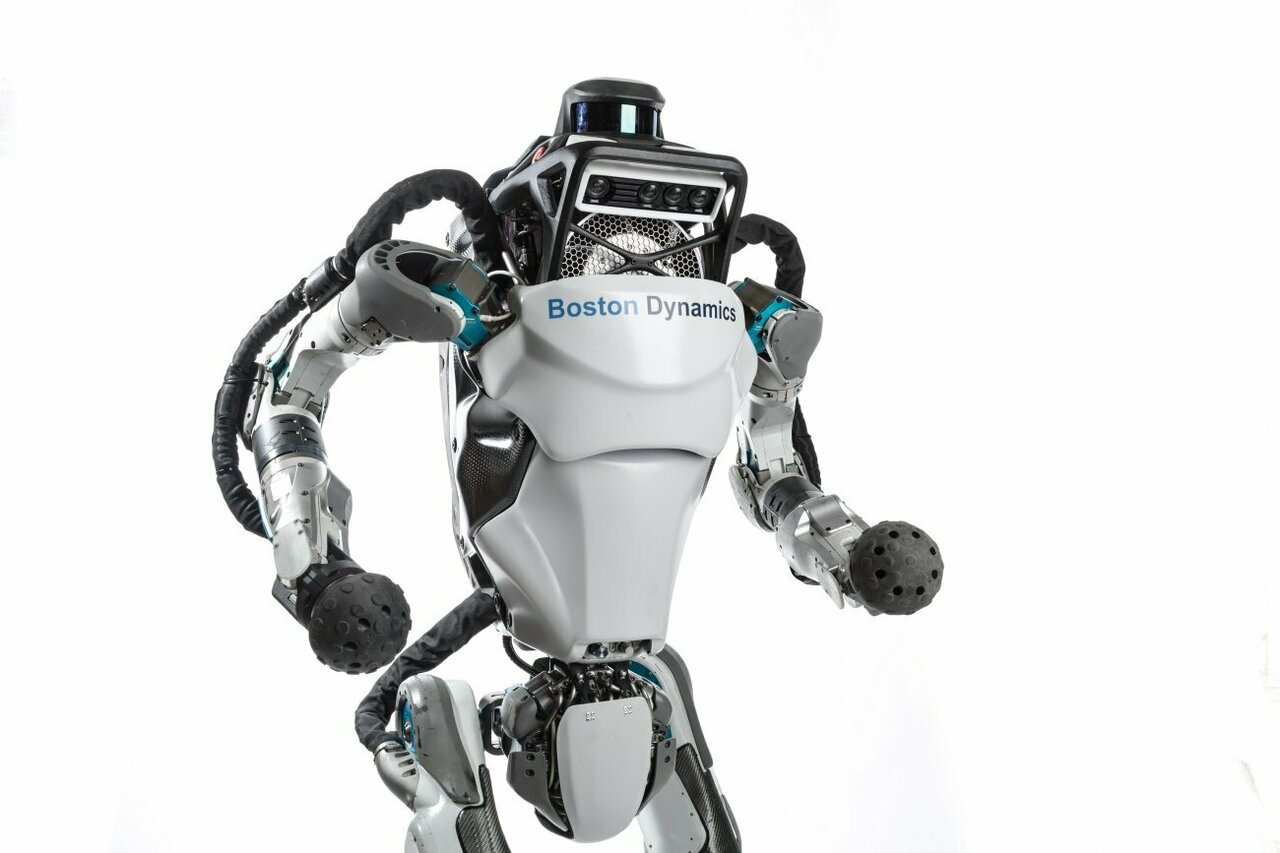
\includegraphics[width=\columnwidth]{robotics.jpg}\\
		\centering{Robotics}%
	\end{subfigure}\hfill
	\begin{subfigure}[t]{0.3\textwidth}
		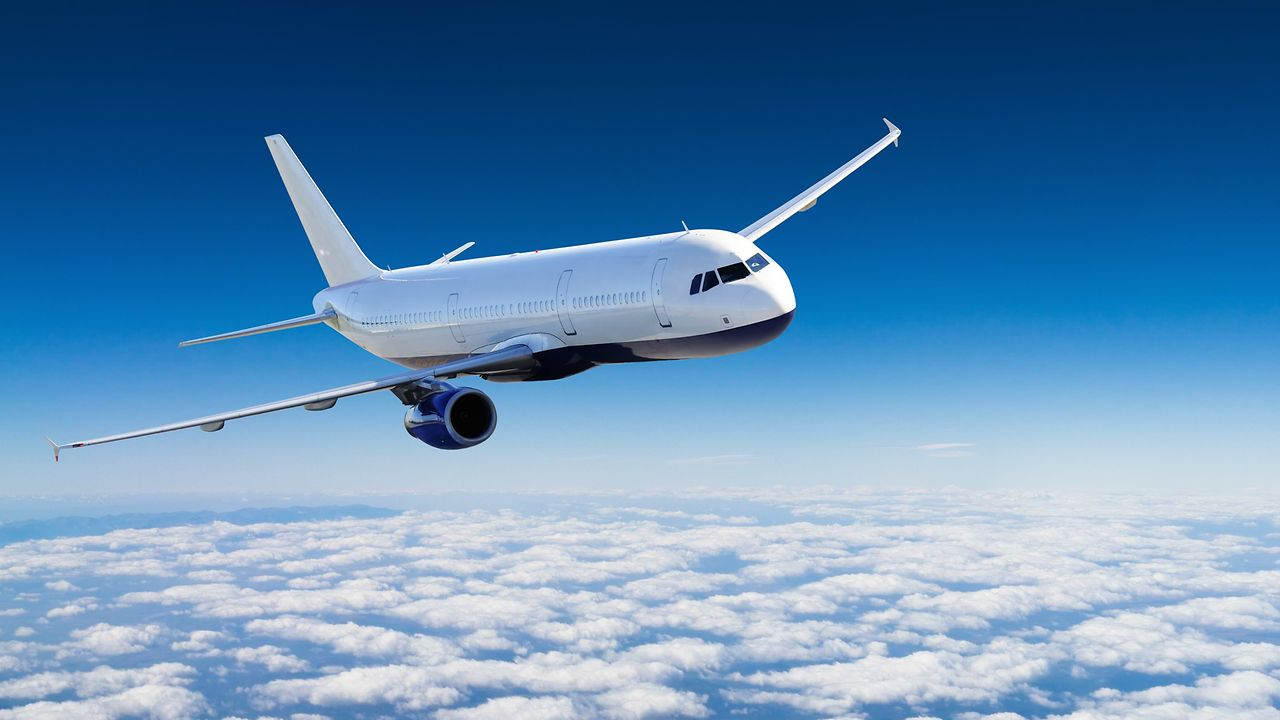
\includegraphics[width=\columnwidth]{aerospace.jpg}\\
		\centering{Aerospace} 
	\end{subfigure}\hfill
	\begin{subfigure}[t]{0.3\textwidth}
		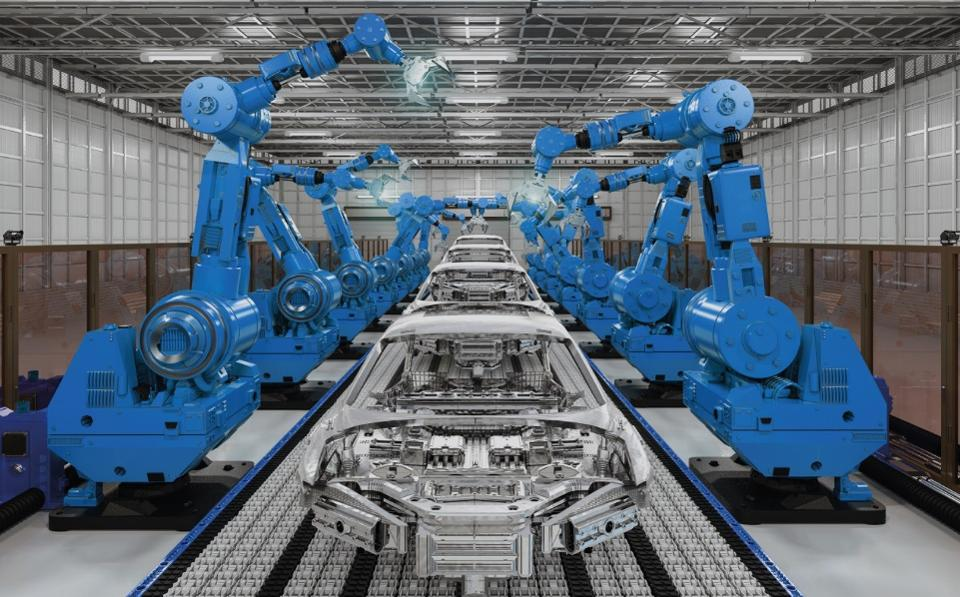
\includegraphics[width=\columnwidth]{manufacturing.jpg}\\
		\centering{Manufacturing}
	\end{subfigure}
\end{figure}

	
\end{frame}

\begin{frame}{The portwings project and its numerical challenges}
	Numerical methods for port-Hamiltonian system should:
	\begin{itemize}
		\item reproduce the physical properties of the problem (conservation laws, symmetries);
		\item preserve the modularity inherithed from the Dirac structure;
		\item work in any spatial dimension;
		\item adaptable to many physical problems (fluid and solid mechanics, electromagnetism, etc.);
	\end{itemize}
\end{frame}

\begin{frame}{Methods for computational simulation}
	\only<1>{
\begin{tcbraster}[raster columns=3, raster equal height]
	\begin{tcolorbox}[width=0.32\textwidth, nobeforeafter, colframe=theme,title=Finite differences]%%
	Pros:
	\begin{itemize}
		\item quadrature-free implementation;
		\item diagonal mass matrices;
	\end{itemize}
	Cons:
	\begin{itemize}
		\item solution is only pointwise;
		\item difficult bcs. implementation;
		\item no Galerkin orthogonality;
	\end{itemize}
	\end{tcolorbox} 
	\begin{tcolorbox}[width=0.32\textwidth, nobeforeafter,  colframe=theme,title=Finite volumes]%%
		Pros:
		\begin{itemize}
			\item Exact conservation laws;
			\item incorporates discontinous phenomena;
		\end{itemize}
		Cons:
		\begin{itemize}
			\item low order approximation;
			\item requires Voronoi dual mesh;
		\end{itemize}
	\end{tcolorbox}
	\begin{tcolorbox}[width=0.32\textwidth, nobeforeafter,  colframe=theme,title=Finite elements]%%
		Pros:
		\begin{itemize}
			\item Galerkin orthogonality;
			\item geometric flexibility;
			\item mathematical foundation;
		\end{itemize}
		Cons:
		\begin{itemize}
			\item trouble at high aspect ratio;
			\item convection problems;
		\end{itemize}
	\end{tcolorbox}
\end{tcbraster}
}

\only<2>{
	If the construction is based on the same ideas, these schemes are equivalent:\\
	\vspace{.5cm}
	\fullcite{adler2021}
	\vspace{1cm}
	
	There is no established superior method and all these methods can all provide impressive results.
}
\end{frame}


\begin{frame}{Finite difference implementation of Rayleigh-Taylor instability}
	\begin{figure}
		\centering
		\includemedia[
		label=vidNoRod,
		addresource=/home/andrea/Videos/Videos_PW/Rayleight_Taylor_FDM.mp4,
		activate=pageopen,
		width=10cm, height=5.5cm, 
		flashvars={
			source=/home/andrea/Videos/Videos_PW/Rayleight_Taylor_FDM.mp4
			&loop=true
		}
		]{}{VPlayer.swf}
	\end{figure}
	Source: \url{https://wci.llnl.gov/simulation/computer-codes/miranda}
\end{frame}


\begin{frame}{Finite volume simulation of a flexible wing}
	\begin{figure}
		\centering
		\includemedia[
		label=vidNoRod,
		addresource=/home/andrea/Videos/Videos_PW/flapping.mp4,
		activate=pageopen,
		width=10cm, height=5.5cm, 
		flashvars={
			source=/home/andrea/Videos/Videos_PW/flapping.mp4
			&loop=true
		}
		]{}{VPlayer.swf}
	\end{figure}
	\fullcite{farhat2012}
\end{frame}

\begin{frame}{Finite elements for computational biology}
	\begin{figure}
		\centering
		\includemedia[
		label=vidNoRod,
		addresource=/home/andrea/Videos/Videos_PW/aorta_FEM.mp4,
		activate=pageopen,
		width=10cm, height=5.5cm, 
		flashvars={
			source=/home/andrea/Videos/Videos_PW/aorta_FEM.mp4
			&loop=true
		}
		]{}{VPlayer.swf}
	\end{figure}
	\fullcite{laadhari2017}
\end{frame}

\begin{frame}{What to choose for port-Hamiltonian systems?}
	Papers concerned port-Hamiltonian systems have tried them all:
	\begin{itemize}
		\item Finite elements (exterior calculus\footcite{golo2004hamiltonian,kotyczka2018weak} or vector calculus\footcite{cardoso2020pfem});
		\item Finite volumes\footcite{serhani2017master};
		\item Finite differences\footcite{trenchant2018};
	\end{itemize}
	\vspace{.5cm}
	\onslide<2->{Two important questions:
	\begin{itemize}
		\item Many of these require an implementation from scratch. Do we really need that?
		\item Can we rely on established theoretical results to have a clear guideline and unified analysis of different methods?
	\end{itemize}}
	
\end{frame}



\section{Finite Element Exterior Calculus for port-Hamiltonian systems}


\begin{frame}{Exterior calculus and discretization of PDEs}
\begin{block}{Bridging the gap with existent literature}
	\fullcite{arnold2006acta}
\end{block}

This framework comes with a periodic table of finite elements for unified analysis\footnote{\url{https://sinews.siam.org/Details-Page/periodic-table-of-the-finite-elements}}. 	Some open source librairies were built to implement the FEEC periodic table\footcite{logg2012,rathgeber2017firedrake}.

\only<1>{
\centering
\includegraphics[width=0.6\textwidth]{periodic-table-of-the-finite-elements_cropped.pdf}\\
}

\only<2>{
\begin{block}{On the importance of FEEC}
\textit{"Just as the arrangement of the chemical elements in a periodic table led to the discovery of new elements, the periodic table of finite elements has not only clarified existing elements but also highlighted holes in our knowledge and led to new families of finite elements suited for certain purposes."}
\end{block}
}
\end{frame}


\begin{frame}{On the application of FEEC to port-Hamiltonian systems}
\begin{overlayarea}{\textwidth}{\textheight}

\begin{alertblock}{Why has this framework not been used (yet)?}
The applications of FEEC to pHs raises some difficult points:
\begin{itemize}
	\item \only<2-4>{how to mimic the Dirac structure at the discrete level (exact enforcements of the conservation laws)?} \only<5->{\textcolor{blue}{how to mimic the Dirac structure at the discrete level (exact enforcements of the conservation laws)?}}
	\item \only<3-4>{how to obtain discrete constitutive equations (discrete Hodge operator)?}
	\only<5->{\textcolor{blue}{how to obtain discrete constitutive equations (discrete hodge operator)?}}
	\item<4-> how to implement generic boundary conditions (modular multiphysics modelling)?
\end{itemize}
\end{alertblock}

\end{overlayarea}
\end{frame}

\section{An illustrative example: the wave equation}


\begin{frame}{The scalar wave equation as a toy problem}
From the linearization of mass and momentum conservation, the acoustic wave equation in irrudicible form is obtained
\begin{equation*}
\rho(\bm{x}) \diffp[2]{p}{t} - \div(\bm{T}(\bm{x})\grad p) = 0,  \qquad \bm{x} \in \Omega \subset \bbR^3, \quad p|_{\partial\Omega} =0.
\end{equation*}
$p$ is the pressure, $\rho(\bm{x})$ the density and $\bm{T}(\bm{x}) \in \bbR^{3\times 3}$ the Young modulus.

Standard discretization method (continuos Galerkin):
\begin{equation*}
	\mathbf{M}_\rho \ddot{\mathbf{p}} + \mathbf{K}_{T} \mathbf{p} = 0.
\end{equation*}
What about conservation of energy? Yes, but a Newmark scheme is needed.\\
Mass and momentum conservation? Lost.
\end{frame}



\end{document}